
\section{Learning Optimal Exploration Behaviors}


Motivated by the existence of optimal algorithms for bandits, we aim to leverage these algorithms to improve LLMs for exploration by:  1) incorporating algorithmic guidance during inference (Section~\ref{subsec: guided_support}),
2) teaching optimal exploration through \ad (Section~\ref{subsec: learning_optimal_behavior}). We show that smaller models trained using \ad can even outperform larger models, offering a promising way to efficiently explore with lower inference costs.

Numerous algorithms have been developed to enable efficient exploration in both MAB~\citep{auer2002finite} and CB~\citep{langford2007epoch,li2010contextual} settings. Among these, the Upper Confidence Bound (UCB) algorithm—also known as optimism in the face of uncertainty—stands out for its simplicity and theoretical guarantees\footnote{UCB calculation is the bedrock for many other algorithms, such as Monte-Carlo Tree Search (MCTS), which is often used to improve LLM performance at inference-time~\citep{snell2024scaling}.}. 
We focus on UCB as our optimal exploration algorithm for both MAB and CB. Its clear and interpretable representation of uncertainty and exploration strategy also makes it well-suited for integration with existing LLMs. Our method can, however, generalize to different algorithms easily.

\paragraph{UCB for Multi-Armed Bandit}
For MAB, at time step $t$, given the history $\{a_{t'}, r_{t'}\}_{t'=1}^t$, we define $N_t(a)$ as the number of times that action $a$ has been selected up to time $t$. The empirical mean reward of arm $a$ up to time $t$, denoted as $\hat{\mu}_t(a):=\sum_{t'=1}^t \frac{\mathbf{1}_{\{a_{t'}=a\}}r_{t'}}{N_t(a)}$, represents the exploitation value $V^{\text{exploit}}(a,t)$. The high-probability confidence interval, also known as the exploration bonus, is given by $V^{\text{explore}}(a,t):=\alpha\sqrt{\frac{\log(t)}{N_t(a)}}$ , where $\alpha$ is the hyperparameter controlling the exploration-exploitation trade-off. At each time step, UCB selects the arm that maximizes the sum of the exploitation value and the exploration bonus, thereby choosing the arm with the highest upper confidence bound.

\paragraph{UCB for Contextual Bandit}
In CB, we consider the case of linear payoffs~\citep{li2010contextual,chu2011contextual}, where the expected reward $\mathbb{E}[r^a_t]$ is assumed to be linear w.r.t a $d$-dimensional feature vector $x^a_{t}$, with some unknown coefficient vector
$\theta^{*}$, i.e., $\mathbb{E}[r^a_t|x^a_t]=(x^a_t)^T\theta^{*}$. At each time step, for any arm $a$, the algorithm maintains the design matrix $D_a\in\mathbb{R}^{N_t(a)\times d}$, which represents the feature data for arm $a$ up to time $t$, as well as the corresponding reward vector $r^a\in\mathbb{R}^{N_t(a)}$. It then estimates $\hat{\theta}$ using ridge regression. Moreover, the high-probability confidence interval of the reward estimate $(x^a_t)^T\hat{\theta}$ is given by $\alpha\sqrt{(x^a_t)^T(D^T_aD_a+\lambda I_d)^{-1}x^a_t}$, with $I_d$ being the identity matrix.
Following MAB, the exploitation value is the reward estimate, and the exploration bonus is the confidence bound around it.


\subsection{Inference-time \ag}
\label{subsec: guided_support}
In this section, we explore how to leverage UCB-type algorithms as inference-time support to improve LLM's in-context exploration performance. 

\paragraph{\ag (AG)} As discussed above, UCB-type algorithms operate by explicitly calculating the exploitation value $V^\text{Exploit}$ along with the exploration bonus $V^\text{Explore}$ for each arm, and by selecting the arm that maximizes the sum of the two. These components, $V^\text{Exploit}$ and $V^\text{Explore}$, therefore provide the sufficient textualization needed for LLMs to make optimal decisions.
Specifically, in the MAB setup, during inference time at time step $t$, we provide the LLM with a list of tuples $\big(V^{\text{exploit}}(a,t), V^{\text{explore}}(a,t)\big)$ for each arm $a\in[K]$. This representation is provided alongside  other essential information, such as scenario descriptions, instructions, and the action set. 
For CB, during inference-time, we explicitly maintain the design matrix $D_a$ and response vector $r^a$ for each arm, incorporating past interactions from the LLM up to that time $t$, using this to obtain the exploitation value and exploration bonus. We then provide the LLM with a list of exploitation values and exploration bonus for each arm $a$ at current context $x$, similar to the MAB setup. Additionally, we record the action features $x^a_t$ as well as the reward $r_t$ selected by the LLM, which will be used for the next round of parameter updates. 
Compared with \textbf{SH}, which only provides the empirical mean and the number of times each arm has been pulled, \textbf{AG} directly supplies semantically understandable exploitation values and exploration bonuses. This explicit representation enables the LLM to effectively balance exploitation and exploration.  Theoretically, the LLM only needs to perform addition and argmax, rather than manipulating raw histories to discern the underlying reward distribution (or parameter $\theta$ in CB). Another advantage is that \textbf{AG} is a type of inference-time support that works seamlessly for both MAB and CB, while \textbf{SH} only works on MAB setup\footnote{If we were to perform a similar analysis with LinUCB, \textbf{RH} would correspond to retaining all (context, action, reward) information to estimate the parameter and calculate the uncertainty, while one possibility to realize \textbf{SH} would be to construct the sufficient statistics using running mean and running covariance matrix in LinUCB. However, these statistics are much less interpretable for language models; thus, we do not investigate it.}. 

\subsection{Algorithm Distillation via Demonstration and Fine-tuning}
\label{subsec: learning_optimal_behavior}


We further investigate the possibility of enhancing LLM exploration by leveraging a set of trajectories generated by an oracle exploration algorithm in the BanditBench environment. 
This approach, called \emph{\ad}, aims to distill the optimal exploration behavior from the oracle algorithm to the LLM.
In particular, we consider two approaches: \emph{in-context few-shot demonstration} and \emph{oracle behavior fine-tuning}, both utilizing expert trajectories generated by the oracle algorithm. 
Compared with \ag (\textbf{AG}), these approaches do not require an understanding of the oracle algorithms, nor do they require generating sufficient statistics based on oracle algorithms; thus, they can also be applied to black-box algorithms. 



\paragraph{Oracle Trajectory Generation} 

We use UCB as the oracle algorithm to generate the trajectories.
Following the notations defined in Section~\ref{sec: icdm}, the trajectories are in the form of tuples of $( \phi(H^{\text{UCB}}_t), a^{\text{UCB}}_t)$, where each tuple pairs the transformed representation of the history at time $t$ and the action $a^{\text{UCB}}_t$ from UCB.
For MAB, we create trajectories from reward distributions that \textit{differ} from those used in evaluation. This assesses the LLM's ability to generalize across different bandit instances with the same underlying scenario but varying \textit{action descriptions} and \textit{action-reward mappings}.
We further control the data generation process by varying: (1). \emph{Action Description}: trajectories are generated from either "Video" or "Clothes" action descriptions;
(2). \emph{Difficulty}: we control the reward gap in the Bernoulli bandit to create "easy" or "hard" instances;
(3). \emph{Trajectory Textualization}: trajectories are represented either as \RH or \AG.
For CB, we use a fixed dataset and evaluate the LLM's performance on a held-out set of users. While these users are unseen during training, their profiles and preferences remain within the distribution of the training data. This evaluates the LLM's ability to leverage prior knowledge for effective exploration.  In CB, we only vary the trajectory representation (\RH or \AG).
In both MAB and CB, each trajectory consists of a sequence of exploration steps: 300 steps for MAB with $K=5$ arms, 1000 steps for MAB with $K=20$ arms, and 200 steps for CB. 
We generate 50 trajectories for 2 MAB domain configurations (the easiest and the hardest configuration) with 2 trajectory textualizations, and 200 trajectories for CB with 2 trajectory textualization . This results in 4 \ad datasets for MAB and 2 datasets for CB. 


\paragraph{In-Context Few-Shot Demonstration}

We first study whether demonstrating oracle exploration trajectories from UCB as few-shot examples can improve the LLM's ability to perform robust exploration in bandit tasks. 
A key challenge in applying few-shot learning to decision-making tasks like MAB is the increasing context length. Unlike supervised learning, where context is typically fixed, bandit actions depend on the entire past history or condensed history, which either grows linearly with $T$ (steps) or $K$ (actions). This poses a challenge for LLMs, as their ability to effectively utilize information can degrade with longer contexts. 
We sample 5 oracle trajectories from UCB into the LLM context window as demonstrations. Our goal is to see whether the optimal exploration demonstrations can lead to improved exploration performance. Detailed demonstrations are provided in Appendix~\ref{app_subsec: few_shot}.

\paragraph{\oft (OFT)}

While in-context few-shot demonstrations offers an inference-time approach to guide the LLM's exploration strategy, fine-tuning allows us to directly optimize the model's parameters for the task. In this approach, we utilize the UCB-generated trajectories as training data to adjust the LLM's internal representations and decision-making mechanisms.
Specifically, we fine-tune the LLM by framing the exploration problem as a language modeling task, where the goal is to predict the next action in the sequence. This is achieved by maximizing the log-likelihood of the UCB actions given the history of interactions:
\begin{equation}
    \loss_{\text{OFT}}(\pi) = -\E_{( \phi(H^{\text{UCB}}_t), a^{\text{UCB}}_t) \sim \data_{\text{OFT}}} 
    [ 
    \log \pi(a^{\text{UCB}}_t|\phi(H^{\text{UCB}}_t))
    ],
\end{equation}
where $\pi$ represents the LLM's policy that we aim to optimize.
This formulation encourages the LLM to learn the underlying patterns and decision-making logic embedded within the UCB trajectories. By predicting the next action in the sequence, the LLM effectively internalizes the optimal exploration strategy demonstrated by the UCB algorithm. 

Optimal Behavior Fine-tuning (OFT) and Behavior Cloning (BC)~\citep{pomerleau1991efficient} share many similarities. However, they are not the same. Although both approaches rely on maximum-likelihood learning, their objectives are different: OFT seeks to encode a dynamic, iterative refinement process, while BC focuses on replicating static behavior. OFT is designed for algorithm distillation, focusing on capturing a sequence of self-improvement behaviors, and generalization across any new test domains. In contrast, BC aims to learn a policy by mimicking a static policy, with no iterative improvement between trajectories.

This difference becomes very clear when we work through this example. Given a policy $\pi$, if our goal is to learn a policy $\hat \pi$ that perfectly mimics the behavior of $\pi$, then we will create a behavior cloning dataset $\gD_{\text{BC}}$, by collecting this policy $\pi$'s interaction with the environment. In this dataset, for the same state $s$, the policy remains unchanged, which the means $\pi(a|s)$ remains the same in the entire dataset given the same state $s$. However, if our goal is to learn to mimic the \textit{improvement} of this policy $\pi$ as it interacts with the environment -- note that the policy improves after a policy improvement operation (e.g., policy gradient update, or q-value update), we are constructing a dataset $\gD_{\text{OFT}}$ from a set of policies: $\{\pi_1, \pi_2, ..., \pi_{*}\}$. This means, given the same state $s$, the action to take will change: $\pi_i(a|s)$, depending on whether this is an early or a late trajectory of this dataset. In order to encode the policy change $i$, the prediction target is $a$ given the current state $s$ and all the previous experiences that were used to improve this policy.


\subsection{Empirical Evaluations}
\label{subsec: eval_and_baselines}
In this section, we empirically evaluate LLMs' in-context exploration capabilities, using BanditBench. We begin with introducing the setup, baselines and metrics in Section~\ref{subsubsec: setup}. Following this, in Section~\ref{subsubsec: results}, we analyze the performance of inference-time guided support, in-context few-shot demonstration and oracle behavior fine-tuning across various experimental settings, as well as models of different sizes. Additionally, we perform extensive ablation studies on the impact of task difficulty, textual representation of the oracle trajectories, and inference-training representation alignment.
\subsubsection{Setup and Baselines}
\label{subsubsec: setup}
\paragraph{Setup} We evaluate the in-context exploration capabilities of various LLMs, including Gemma-2B, Gemma-9B~\citep{team2024gemma}, Gemini 1.5 Flash, and Gemini 1.5 Pro~\citep{reid2024gemini}, on 16 MAB tasks (Table~\ref{tab:mab_config}) and 2 CB tasks.
For MAB tasks, the interaction horizon ($T$) differs based on the size of the action space ($K$): we use $T=1000$ for $K=30$ and $T=200$ for $K=10$.
All CB tasks use a constant horizon of $T = 200$ steps.
To ensure statistical significance of the results, we conduct 30 independent runs for each experimental setup.

\paragraph{Baselines} We consider two baselines: Raw History (\textbf{RH}) and Summarized History (\textbf{SH}), as suggested in~\citet{krishnamurthy2024can}.
For CB, as we discussed before, there is no trivial analogue of \textbf{SH}; thus, we focus solely on \textbf{RH} for CB tasks in this study as the baseline. 

\paragraph{Metrics}
We report the relative performance of each model, aggregated across all environment configurations. Simply averaging cumulative rewards across environments of different reward distributions and horizons however, obscures the comparison. We instead use the \emph{pairwise} win-rate to compare the performances. We have 16 configurations for MAB and evaluate 32 models (4 LLMs crossed with different methods), and 2 configurations for CB with 14 models (2 LLMs crossed with different methods).  The list of all the models is provided in Appendix~\ref{sec:app:model_full_list}. For each configuration, we compute the cumulative reward over 
$T$ steps and collect a distribution of cumulative rewards from 30 independent trials. We then calculate the pairwise win-rate by applying a Student's $t$-test on the reward distributions of any pair of configurations to determine if they are statistically significantly different, with a significance level of $p<0.05$. If one model has a significantly higher reward than the other, we consider it a win. If the difference is not statistically significant, the result is deemed inconclusive and not counted as a win.
For each model, we calculate its win rate against every other model across all configurations. The \emph{\awr} for a specific model is then the percentage of superior performance over all models, crossed with methods and configurations. 


\subsubsection{Results and Ablation studies}
\label{subsubsec: results}

\paragraph{Overall Performance Comparison} 

Figure~\ref{fig:fewshot_sft_result} presents a comparative overview of in-context few-shot demonstration, oracle behavior fine-tuning, and inference-time algorithmic guidance performance across various model sizes and training configurations. Detailed numbers are reported in Table~\ref{tab:inference_time_algs} and~\ref{tab:training_time_algs}.
Few-shot demonstrations exhibited contrasting effects on Gemini-1.5 Flash and Pro. While few-shot learning boosts the performance of Flash beyond the best history contextualization setup, it hurts Pro's performance in both MAB and CB. Aligned with the observations in~\citet{zheng2024natural,guo2025deepseek}, our hypothesis is that few-shot examples we manually crafted could disrupt the CoT structure in larger models, which requires the few-shot examples to be carefully tuned in order to be helpful.
Further analysis reveals the remarkable effectiveness of oracle behavior fine-tuning. It significantly outperforms both few-shot and baseline approaches in both MAB and CB across all model sizes, even larger ones.
This robust improvement highlights the effectiveness of directly optimizing model parameters for the exploration task. Notably, the best fine-tuned Gemini-1.5 Flash model surpasses even the Gemini-1.5 Pro model, highlighting its potential as a key technique for enhancing LLM exploration capabilities.

\begin{table}[]
\small
\centering
\begin{tabular}{@{}lcccc|cc@{}}
\toprule 
\multirow{2}{*}{Inference-Time Support}  & \multicolumn{4}{c}{\textbf{Multi-Armed Bandit}} & \multicolumn{2}{c}{\textbf{Contextual Bandit}} \\ \cmidrule(l){2-7}  %\midrule  %
                 & Gemma-2B & Gemma-9B      & Flash   & Pro  & Flash   & Pro   \\ \midrule
\rah (\RH)          & 7.6 & 10.5       & 27.7              & 45.5           & 0.0                 & 7.1            \\
\sh (\SH)  & 10.5 & 5.3         & 34.8              & 60.0           & --                 & --               \\ 
\ag (\AG)  & 4.9 &  4.1         & 32.2              & 59.6           & 46.4              & 64.3            \\ \midrule
UCB / LinUCB & \multicolumn{4}{c|}{90.6} & \multicolumn{2}{c}{96.4}  \\
\bottomrule
\end{tabular}
\caption{\footnotesize{\AWR (\%) of different inference-time support. Flash and Pro refer to Gemini-1.5 Flash and Pro respectively. Unlike \SH, \AG can work for both MAB and CB. Refer to Section~\ref{subsec: guided_support} for details.}}
\label{tab:inference_time_algs}
\vspace{-0.2cm}
\end{table}

\begin{table}[]
\small
\centering
\begin{tabular}{@{}lcc|cc@{}}
\toprule
 & \multicolumn{2}{c}{\textbf{Multi-Armed Bandit}} & \multicolumn{2}{c}{\textbf{Contextual Bandit}} \\ \cmidrule(l){2-5} 
 Few-shot Demonstrations                         & Flash   & Pro  & Flash   & Pro   \\ \midrule
\rah (\RH)                & 27.5              & 39.1           & 3.6                 & 7.1            \\
\ag (\AG)         & 50.2              & 56.4           & 60.7              & 25.0           \\ \midrule
\oft  \\  \midrule 
\rah (\RH) & \textbf{65.6} & --- & 28.6 & --- \\
\ag (\AG) & 28.3 & --- & \textbf{89.3} & --- \\ \midrule 
UCB / LinUCB & \multicolumn{2}{c|}{90.6} & \multicolumn{2}{c}{96.4}  \\
\bottomrule
\end{tabular}
\caption{\footnotesize{\AWR (\%) of different \ad methods. Flash and Pro refer to Gemini-1.5 Flash and Pro respectively. Best achieved performances are highlighted. In this table, the history textualization used in oracle trajectory and inference-time support are the same. We conduct a few ablations in Figure~\ref{fig:cb_ablations}.}}
\label{tab:training_time_algs}
\end{table}


\begin{table}[h]
\small
\centering
\begin{tabular}{@{}lcccc@{}}
\toprule
     & Flash (\RH) & Flash (\AG) & Pro (\RH) & Pro (\AG) \\ \midrule
MAB, K=5  & \textbf{33.6}     & 26.6     & 48.0   & \textbf{67.6}   \\
MAB, K=20 & 21.9     & \textbf{37.9}     & 43.0   & \textbf{51.6}   \\ \midrule 
CB, K=10 & 0.0 & \textbf{35.7} & 7.1 & \textbf{57.1} \\
CB, K=30 & 0.0 & \textbf{57.1} & 7.1 & \textbf{71.4} \\
\bottomrule
\end{tabular}
\caption{\footnotesize{Situations where \ag significantly outperforms \rah during inference.}}
\label{tab:ag_helped}
\vspace{-0.5cm}
\end{table}

\paragraph{\ag Helps on Complex Environments}

We observe consistent improvements when transitioning from \RH to \AG in two scenarios: (1) larger models like Flash and Pro, and (2) more complex scenarios, such as contextual bandits. Table~\ref{tab:ag_helped} shows that \AG provided consistent help when the number of actions is large for both Flash and Pro models. We hypothesize that providing \AG is crucial when the action space is large or when decision scenarios are complex.

\paragraph{Impact of Task Difficulty}

We examine whether the choice of oracle trajectories used in both few-shot demonstration and oracle behavior fine-tuning affects the model's performance during inference. To investigate this, we select trajectories from two extreme setups. The easiest setup involves \emph{(Bernoulli, Video, Large $\Delta_{min}$, $K=5$)}, denoted as $D_{\text{easy}}$, with \AG. Conversely, the hardest setup, denoted as $D_{\text{hard}}$ utilizes \emph{(Bernoulli, Clothes, Small $\Delta_{min}$, $K=20$)}, with \RH.  
Figure~\ref{fig:mab_domains_sft_fewshot} illustrates that the choice of oracle trajectories significantly impacts the model's performance, with a surprising contrast between the two \ad methods.
Few-shot demonstration achieves a higher win-rate when using $D_{\text{easy}}$ as demonstration (50.2) compared to when using $D_{\text{hard}}$ (43.0). This suggests that the limited examples provided in the demonstrations may be insufficient for the model to effectively utilize them under the higher complexity and subtle reward signals of the harder task. 
Conversely, fine-tuning exhibits the opposite trend, with a higher win-rate when trained on $D_{\text{hard}}$ (65.6) compared to $D_{\text{easy}}$ (54.5). 
This implies that fine-tuning, with its extensive training data, might be overfitting to the specific nuances of the training distribution, leading to poor generalization when faced with a different task structure.

\paragraph{Impact of Contextualization}
We further investigate the effect of contextualization in oracle trajectories. We consider two representations in MAB: \RH and \SH.
Results in Figure~\ref{fig:mab_text_rep_sft_fewshot} reveal a  clear contrast in how these representations affect the two \ad methods. For few-shot demonstration, \SH leads to significantly better performance (50.2\% win-rate) compared to \RH (27.5\% win-rate).  This suggests that providing concise, informative summaries of optimal exploration behavior is more effective for few-shot learning than presenting the complete raw history. 
On the other hand, fine-tuning exhibits the opposite trend. \RH has a substantially higher win-rate (65.6) compared to \SH (28.3). This indicates that fine-tuning benefits from the richer information present in complete action-reward sequences, allowing it to learn more nuanced patterns of the optimal exploration strategy.
These contrasting preferences for textual representation in oracle trajectories highlight the nuanced ways in which fine-tuning and few-shot learning interact with different types of information. 
Furthermore, in CB, we observe a significant impact of incorporating \AG information into the oracle trajectories for fine-tuning, leading a dramatic improvement in win-rate, rising from 28.6 to 89.3 (Figure~\ref{fig:cb_fewshot_sft_ablations}).
This suggests that providing LLMs with explicit insights, in addition to the complete action-reward sequence, enhances its ability to learn and generalize the optimal exploration strategy in the CB environment. 

\begin{figure*}
\centering
\begin{subfigure}[t]{0.3\textwidth}
\centering
% \vspace{-24mm}
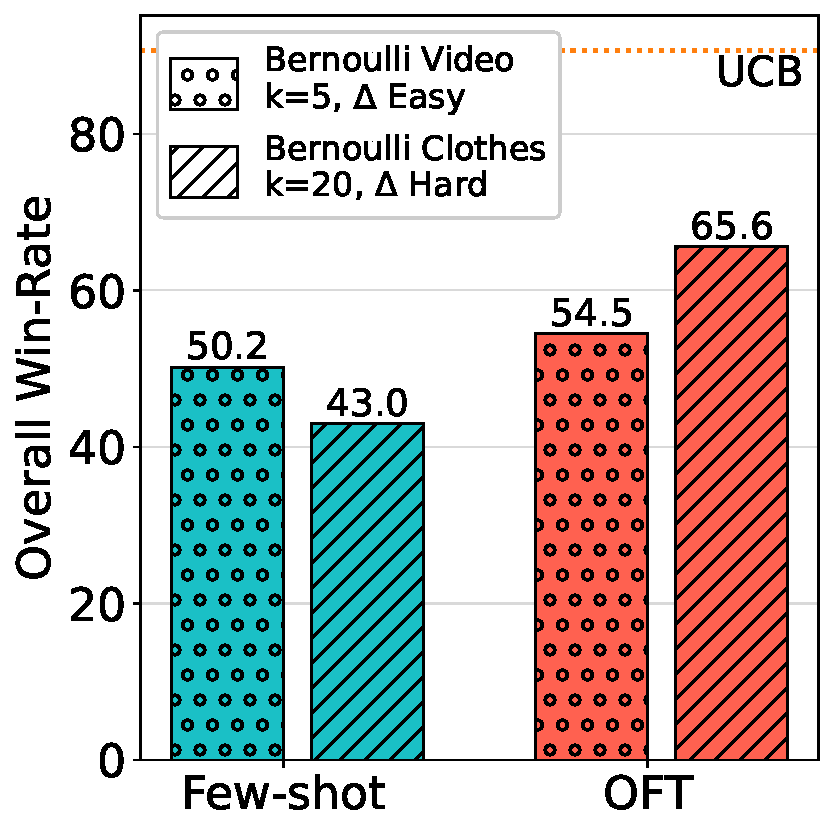
\includegraphics[width=\linewidth]{figures/domains_sft_fewshot.pdf} 
\caption{Task Difficulty (MAB).}
\label{fig:mab_domains_sft_fewshot}
\end{subfigure}
\quad
\begin{subfigure}[t]{0.3\textwidth}
\centering
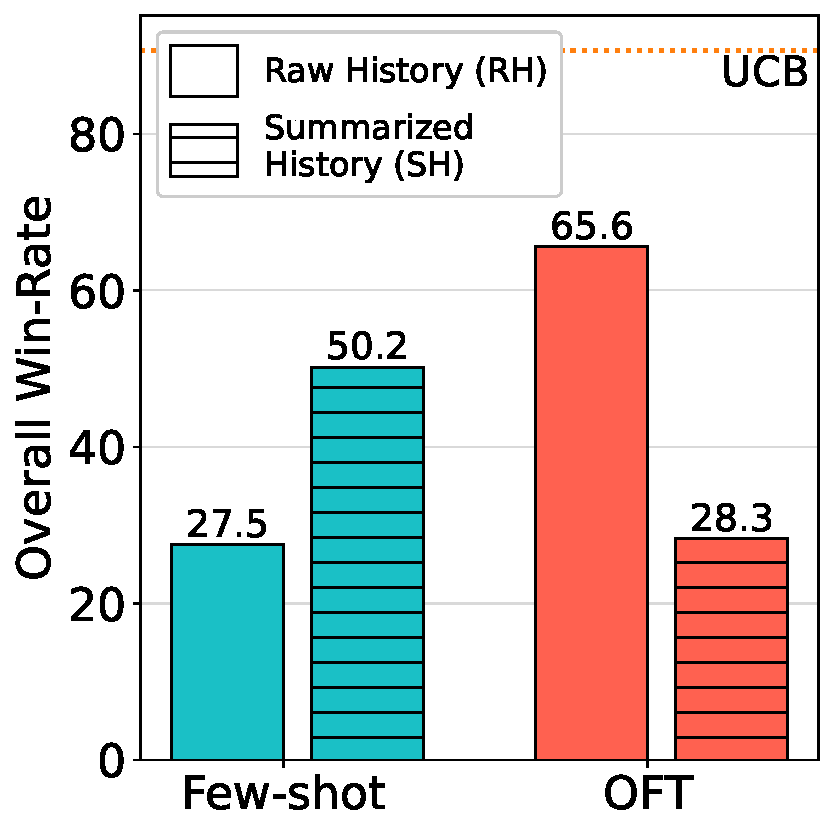
\includegraphics[width=\linewidth]{figures/mab_text_rep_sft_fewshot.pdf}
\caption{History Context Representation, \RH vs \SH (MAB).}
\label{fig:mab_text_rep_sft_fewshot}
\end{subfigure}
\quad
\begin{subfigure}[t]{0.3\textwidth}
\centering
% \vspace{-24mm}
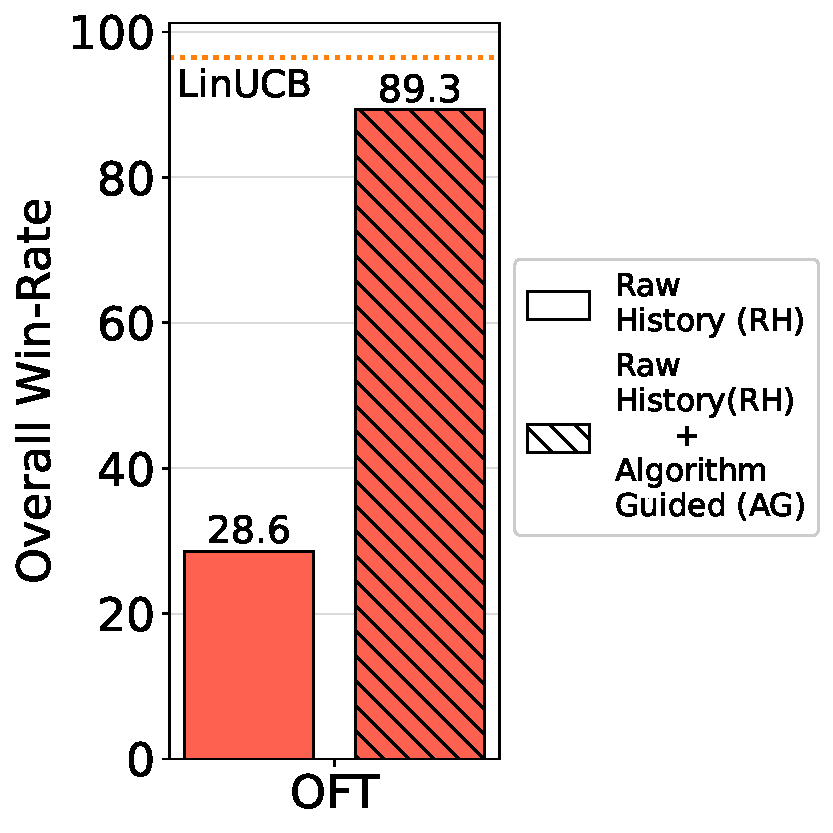
\includegraphics[width=\linewidth]{figures/cb_text_rep_sft_fewshot.pdf}
\caption{History Context Representation with and without \AG (CB).}
\label{fig:cb_fewshot_sft_ablations}
\end{subfigure}
\caption{\footnotesize{\textbf{Impact of task difficulty and textual representation on \ad.} This figure examines how different factors, such as task difficulty and textual representation of oracle trajectories, influence the effectiveness of \ad on the LLM's exploration capabilities. All results are based on Gemini-1.5 Flash model.}}
\label{fig:fewshot_sft_ablations}
\vspace{-4mm}
\end{figure*}

\paragraph{Algorithm Distillation Generalizes}
We also conducted experiments to evaluate the distillation algorithm's ability to generalize from smaller to larger action spaces (i.e., easy-to-hard domain generalization).  This analysis offers insights into the scalability and adaptability of our approach to more complex domains, such as real-world recommendation systems and other complex decision-making problems. We report this in Table~\ref{tab:ad_generalizes}. Using few-shot demonstrations or doing oracle behavior fine-tuning from 
simple-domain trajectories collected (Bernoulli, Easy, K=5) can indeed learn exploration strategies that generalize to a harder domain (Bernoulli, Hard, K=20).

\begin{table}[h]
\small
\centering
\begin{tabular}{@{}lccc@{}}
\toprule
\begin{tabular}[c]{@{}c@{}}MAB\\Hard\end{tabular} & \begin{tabular}[c]{@{}c@{}}Flash \\(\SH)\end{tabular}  & \begin{tabular}[c]{@{}c@{}}Flash + Few-Shot (\SH) \\ ($\data_\text{easy}$ on K=5)\end{tabular} & \begin{tabular}[c]{@{}c@{}}Flash + OFT (\RH) \\ ($\data_{\text{easy}}$ on K=5)\end{tabular} \\ \midrule
K=20 & 34.0\% & 43.0\%                            & 48.4\%                       \\ \bottomrule
\end{tabular}
\caption{\footnotesize{\textbf{Easy-to-Hard Generalization}: We collect distillation data from easy bandit tasks to learn the exploration behavior and evaluate on hard bandit tasks. History representation during evaluation is in parentheses.}}
\label{tab:ad_generalizes}
\end{table}

\begin{figure*}
\centering
\begin{subfigure}[t]{0.4\textwidth}
\centering
% \vspace{-24mm}
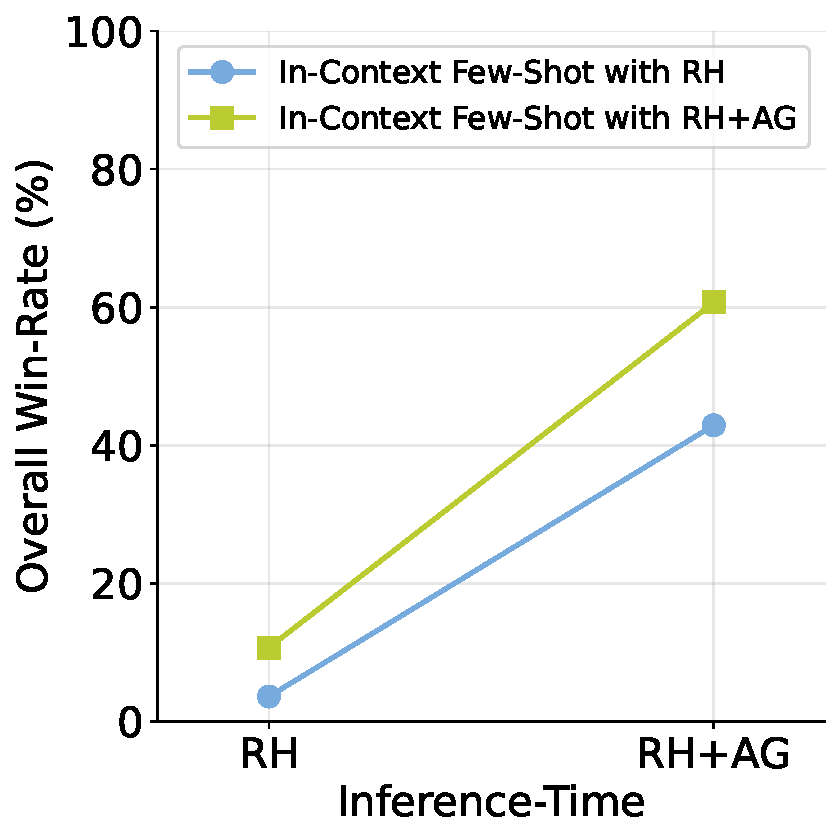
\includegraphics[width=\linewidth]{figures/few_shot_inference_time.pdf} 
\caption{In-Context Few-Shot Demonstration}
\label{fig:few_shot_inference_time}
\end{subfigure}
\quad
\begin{subfigure}[t]{0.4\textwidth}
\centering
% \vspace{-24mm}
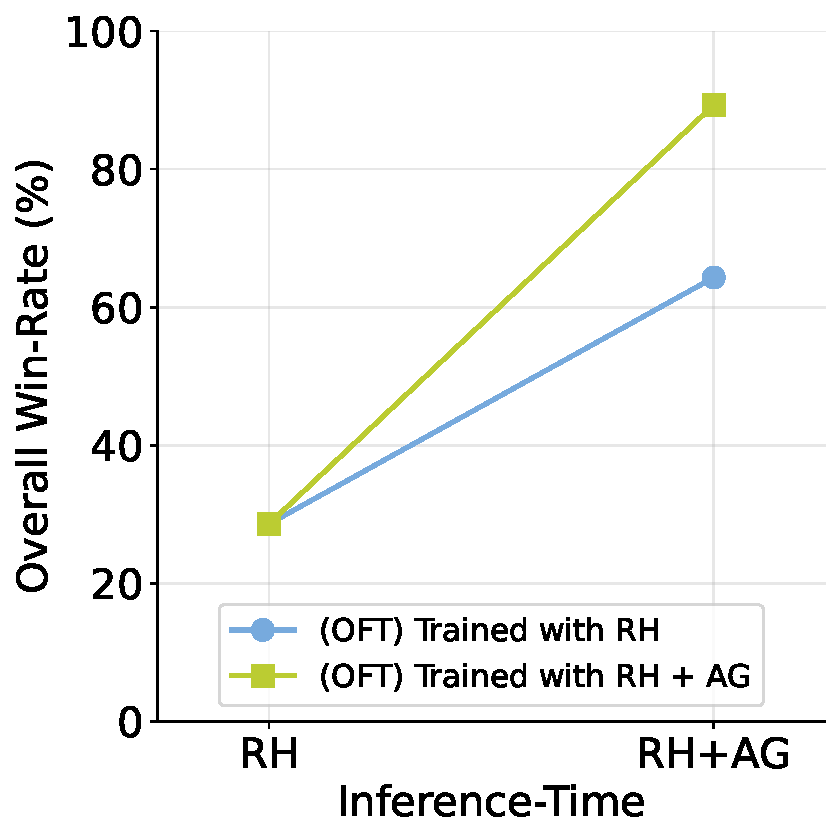
\includegraphics[width=\linewidth]{figures/trained_inference_time.pdf}
\caption{Oracle Behavior Fine-Tuning}
\label{fig:trained_inference_time}
\end{subfigure}
\caption{\footnotesize{\textbf{The Impact of Context Representation in In-Context Examples and Fine-Tuning Data at Inference Time.}} We vary the context representation during ``learning'' (in-context and weight fine-tuning) and provide or withhold information during inference. Providing \AG during inference will always increase the model's performance. Providing it during learning allows the model to maximally leverage such infomation.}
\label{fig:cb_ablations}
\vspace{-4mm}
\end{figure*}

\paragraph{Impact of Training and Inference-time Representation Alignment}
Our experiments also reveal an interesting interplay between the presence of algorithm-guided information (\AG) in both the oracle \emph{trajectories} and \emph{inference}. In the CB setting, providing \AG during inference consistently boosts performance, regardless of whether \AG was used in oracle trajectories. This is clearly demonstrated in Figure~\ref{fig:cb_ablations}, where the right column (with \AG at inference time) exhibits higher win-rates than the corresponding left column across all training conditions. This suggests that the LLM can effectively leverage this information even if it wasn't explicitly trained on it, highlighting the inherent value of structured guidance for decision-making.
Furthermore, we observe that incorporating \AG into few-shot demonstrations improves exploration even when \AG is absent during inference (e.g., Fewshot, \RH 3.6 to \RH+\AG 10.7). This indicates that exposing the LLM to \AG in oracle trajectories, even in a limited capacity, can enhance its ability to extract relevant patterns from \RH.  We hypothesize that \AG helps the LLM learn to focus on the most informative aspects of the history, which generalizes even when \AG is not provided during inference.

\paragraph{Optimality Analysis of Exploration}
We use two metrics to capture high-level exploration behaviors: (1) \textbf{MinFrac}, proposed by \citet{krishnamurthy2024can}, captures the fraction of pulls allocated to the least-selected arm. An ideal algorithm should exhibit high \textbf{MinFrac} during early exploration and gets lower as $t$ increases, indicating effective exploration; (2) \textbf{OptFrac}, tracks the percentage of times the optimal arm is pulled. Ideally, this percentage should increase as the process progresses, indicating the model's ability to self-improve. Using Flash model and Bernoulli bandit configurations as an example in Table~\ref{tab:exploration_optimality}, we see that with \AG, the Flash model on average explores more compared to \SH and have higher success at identifying the best arm.

\begin{table}[h]
\small
\centering 

\begin{tabular}{@{}llllll@{}}
\toprule
\textbf{MinFrac} / $t$ Step         & 100-th   & 250-th   & 500-th   & 750-th   & 1000-th                                 \\ \midrule
UCB & 82.3\% & 48.6\% & 27.8\% & 19.6\% & 15.3\% \\
Flash (\SH)  & 10.2\% & 4.2\% & 2.1\% & 1.4\% & 1.1\%  \\ 
Flash (\AG)  & 11.3\% & 4.5\% & 2.3\% & 1.5\% & 1.1\% \\ \midrule 
\textbf{OptFrac} \\ \midrule 
UCB & 32.7\% & 49.4\% & 58.7\% & 62.6\% & 65.0\% \\
Flash (\SH) & 9.3\% & 10.1\% & 10.4\% & 10.6\% & 10.7\% \\
Flash (\AG) & 14.4\% & 15.6\% & 16.3\% & 16.6\% & 16.8\% \\
\bottomrule
\end{tabular}
\caption{\footnotesize{\textbf{Optimality of Exploration}: We show the measures on the $t$-th step along the progression of exploration, averaged across Bernoulli MAB configurations. Full version with more models in Table~\ref{tab:full_optimality_minfrac} and \ref{tab:full_optimality_optfrac}.}}
\label{tab:exploration_optimality}
\vspace{-5mm}
\end{table}

While a model might achieve high performance by chance—e.g., consistently selecting the optimal arm without deliberate exploration—we examine its behavior more closely using two metrics. \textbf{OptFrac} measures how often the optimal arm is chosen, revealing whether the model increasingly favors the best option. As shown in Table~\ref{tab:exploration_optimality}, UCB's OptFrac steadily rises over time (32.7\% $\rightarrow$ 65.0\%), while Gemini-1.5 Flash remains nearly flat (9.3\% $\rightarrow$ 10.7\%), suggesting limited adaptation. To assess directed exploration, we use \textbf{MinFrac}, the fraction of pulls allocated to the least-selected arm. UCB shows a desirable decline (82.3\% $\rightarrow$ 15.3\%), indicating early broad exploration followed by exploitation. In contrast, Gemini-1.5 Flash starts low and drops quickly (11.3\% $\rightarrow$ 1.1\%), implying minimal directed exploration throughout. Together, these metrics demonstrate that Gemini's performance is not driven by meaningful exploration. More discussion in Appendix~\ref{app:sec:optimality}.

